

%1a/b Is Optimization possible?
%       1a. Construction of tests from diverse experimental sources (I wrote the neuroelectro api and its use in neuronunit, and wrote the original Allen one, but you have put in work to create runnable tests from these and other sources).  This is in a sense a method, but you can still report that these tests are runnable, even outside of optimization.
%       1b. Simulated data tests of optimization.  What works?  What doesn’t?  Why (briefly, saving some for discussion)?  NeuroElectro vs Allen also belong here, and fits in with 1a.  You should talk about model means vs means of models (or whatever we are calling it) here, if you have the results for it or think you can in 3 weeks.  

       %You can talk about rippled error surfaces — this is such a deep technical detail that I wouldn’t spend a lot of time on it.  In other words it may be important but it will be almost impossible to follow even if written well.

Two Experimental Data Types: Spike Feature Experiments, versus Electro-physiology reports.



\subsection{Useable NeuronUnit Allen Constraints}
We created an Allen cell-types API, the API allows one to create neuronunit tests from a data base of experimental cellular recording waveforms. In order to create NeuronUnit tests, one must query the cell-types database, impose a new organization on the data, extract relevant features, and convert model features to NeuronUnit tests. A similar API was created in order to render BlueBrain Project waveforms, eligible for NeuronUnit testing, such that the both the BlueBrain \cite{toledo} and Allen Cell-type data could then guide model fitting. %Tests obtained via the Allen API, were designed to execute inside a NeuronUnit and BluePyOpt frameworks.  

%experiment to NeuronUnit test

One can see the APIs being creating novel NeuronUnit tests here \url{https://github.com/fun-zoological-computing/BluePyOpt/blob/master/examples/bpo_nu_fusion/allen_efel_nu_deployed_tests_only-thesis.ipynb}
%Construction of tests from diverse experimental sources 
%My allen API is perhaps scattered. Allen API.
%Which is the best model.
In order to optimize reduced models, it was first necessary to develop optimizer-friendly implementations of these models. As described in methods, I developed four different optimizer friendly models: Izhikevich model (spanning seven regimes), Adaptive Exponential Integrate and Fire model, and General Leaky Integrate and Fire Model, additionally I included a slower traditional conductance based model, to make some comparisons.

The range of tests available for optimization in NeuronUnit was also incomplete, as it was limited to the passive membrane properties or the shapes of single action potentials.  In order for model output to reflect experimental data, it was also necessary that the timing and patterns of action potentials be assessed and tested. 

I developed the ability for EFEL features to be calculated on NeuronUnit models, as well as tests based on FISlope in Allen celltypes which were coalesced into dedicated EFEL Allen Data test sets. This required both the extraction of novel features EFEL and novel test types: [ISI, AHP\_depth, adaption ratio etc.]. As described in the introduction, knowledge of error surfaces is helpful for garunteeing a good optimization result. Through human examination of resulting error surfaces, it was found that some of these tests were also intractable, because they depended on measurements that were changeable relative to some other changeable measurement inside the cell usually $max(\frac{dV_{m}}{dt})/10$.

Multi-core and or multi-threaded optimization requires that information about model properties be shareable across various processor threads. However, some common data types contain information that is not shareable between CPUs, and they must be translated into a globally sharable framework. I created a class Data Transport Container, that could contain be used to circulate only essential data, in a more primitive but shareable form. This class was also acculated useful helpful methods such as retreiving default model parameters.

%\subsection{Standard Error of the Mean}
%For
In order to both control optimization parameters and visualize optimization results, I also developed a web application, the application requires no programming skill to use, and it allows a user of the to select among multiple cell specific constraints, and multiple model types. Once the user has specified enough parameters to define an optization job, the job can launch, and then return interactive results to the user when the optimization job is complete typically in minutes.


The range of tests available for optimization in NeuronUnit was also incomplete, especially as it focused on passive membrane properties or the shapes of single action potentials.  In order for model output to reflect experimental data, it was also necessary that the timing and patterns of action potentials be assessed and tested.  Therefore, I developed the ability for EFEL features to be calculated on NeuronUnit models. 

This required both the extraction of novel features [Allen, EFEL, etc.] and novel test types: [ISI, AHP\_depth, adaption ratio etc.] Ultimately, I still found that some tests were intractable, because they depended on measured features, relative to some other changeable measurement inside the cell usually $max(\frac{dV_{m}}{dt})/10.$

Multi-core and or multi-threaded optimization requires that information about model properties be shareable between various processor threads. However, some common data types contain information that is not shareable between CPUs, and they must be translated into a globally sharable framework. I created a class, that could translate and envelope only shareable data to solve this problem.

In order to both control optimization parameters and visualize optimization results, I also developed a web application, the application requires no programming skill to use, and it allows a user of the to select among multiple cell specific constraints, and multiple model types. 
%
%\begin{comment}


\subsubsection{Is Optimization possible?}
Not all data-sets where equally conducive towards optimization with reduced cells. In particular the cerebellum purkinje cell demands a very high current injection value to elicit a rheobase spike, $680pA$, and the reduced cells were generally not able to model this inhibited behavior.

Previously, the INCF created a model data fitting competition, were participants competed to submit models, that were best able to fit membrane voltage from a variety of suprathreshold current injection experiments. In this competition, unlike in this work the best models had to predict spike time. Within the scope of this project, post-optimization, ranking of the different models in terms of their ability to explain the most in-vivo experiments. 

There are some data sources, that no models seem to do well on, however, the majority of experiments cause good fits, and the models should compete with each other.

Over all the tests, including challenging Cerebellar Purkinje cell, and olfactory bulb mitral cell, actually the Izhikevich model was the top ranking cell, as it was able to perform the best all-round fits. However if you were to remove those two data sets, and evaluated on the remaining 6-8 out of data sets, the Adaptive Exponential model would be a better fit.


%
%\begin{comment}

%\subsection{Neocortical Layer 4/5 Pyramidal Cell Test Suite}
\subsubsection{2a}

%Direct Quote: "widening of the spike shape, decrease of the firing rate and change in the interspike interval distribution". %All these single unit waveform shapes increased their width with temperature.\cite{goldin2017temperature}

It is possible that the majority neuroelectro recordings of L5PC, spike width were conducted under room temperature as opposed to body temperature, and the relative cooling may have contracted their spike width.
\cite{goldin2017temperature}

\subsubsection{Conflicts between experimental constraints}

Conflicts between Rheobase value, and other static electrical measurements were observed in NeuroElectro and Allen Cell types measurements. When optimizing against NeuroElectro averaged measurements, and Allen Cell types single cell observations, it was common to experience a conflicted ability for the cell to satisfy all constraints simultaneously. 
Models seemed to have particular difficulty in recapitulating an accurate fit for rheobase, while simultaneously satisfying the larger set of fitness criteria: time constant, input resistance, capacitance and resting membrane potential. There was better agreement between firing rate versus current (FISlope) and the remainder of the electrical observations.

%\subsection{Section 2.1}
%
Note this is a cell from the l5 somatosensory rat, hind leg region, so it is probably not comparable to NeuroElectro Data.
\subsubsection{Performance of Layer 5 Prefrontal cortex Pyramidal Neuron on NeuronUnit tests of model data agreement}
\cite{van2016bluepyopt}
A suite of neuronunit tests containing the tests: rheobase value, membrane voltage time constant ($tau_{m})$, input resistance was computed. This multi-compartment, conductance based model served as a useful benchmark, for us to evaluate the relative performance of reduced model fits.

Significant development work went into making the model eligible to take NeuronUnit tests, by way of creating a specially dedicated NeuronUnit backend, to run this complicated conductance based multi-compartment model originating from the blue brain model \cite{markram2015reconstruction}. The intention is that by making this model interoperable with NeuronUnit the model will be able to amenable to optimization.


\subsection{The Experimental Measurements}

\begin{table}[ht]
\centering
\resizebox{\textwidth}{!}{
\begin{tabular}{lllllllll}
\toprule
name & Hippocampus CA1 pyramidal cell & Cerebellum Purkinje cell & Neocortex pyramidal cell layer 5-6 &      olf\_mit &      623960880 &      623893177 &      471819401 &      482493761 \\
\midrule
RheobaseTest                   &                      189.24 pA &                680.79 pA &                          213.85 pA &          NaN &        70.0 pA &       190.0 pA &       190.0 pA &        70.0 pA \\
InputResistanceTest            &                    107.08 Mohm &              142.06 Mohm &                        120.67 Mohm &  130.08 Mohm &  241.0 megaohm &  136.0 megaohm &  132.0 megaohm &  132.0 megaohm \\
TimeConstantTest               &                        24.5 ms &                      NaN &                           15.73 ms &     24.48 ms &        23.8 ms &        27.8 ms &        13.8 ms &        24.4 ms \\
CapacitanceTest                &                        89.8 pF &                620.27 pF &                          150.58 pF &    235.75 pF &            NaN &            NaN &            NaN &            NaN \\
RestingPotentialTest           &                      -65.23 mV &                -61.59 mV &                          -68.25 mV &    -58.14 mV &       -65.1 mV &       -77.0 mV &       -77.5 mV &       -71.6 mV \\
InjectedCurrentAPWidthTest     &                        1.32 ms &                  0.41 ms &                            1.21 ms &      1.61 ms &            NaN &            NaN &            NaN &            NaN \\
InjectedCurrentAPAmplitudeTest &                       86.36 mV &                 71.23 mV &                           80.44 mV &      68.4 mV &            NaN &            NaN &            NaN &            NaN \\
InjectedCurrentAPThresholdTest &                       -47.6 mV &                -46.89 mV &                          -42.74 mV &     -38.9 mV &            NaN &            NaN &            NaN &            NaN \\
FITest                         &                            NaN &                      NaN &                         0.05 Hz/pA &          NaN &     0.18 Hz/pA &     0.12 Hz/pA &     0.18 Hz/pA &     0.09 Hz/pA \\
\bottomrule
\end{tabular}}
\end{table}


This elaborate biophysical model includes the backpropogating dendritic action potential.
\url{https://github.com/BlueBrain/BluePyOpt/blob/master/examples/l5pc/L5PC.ipynb}
\url{https://github.com/social-hacks-for-mental-health/BluePyOpt/blob/master/examples/l5pc/L5PC.ipynb}


\begin{figure}
\begin{center}


\centering
\begin{subfigure}{.2}
  \centering
    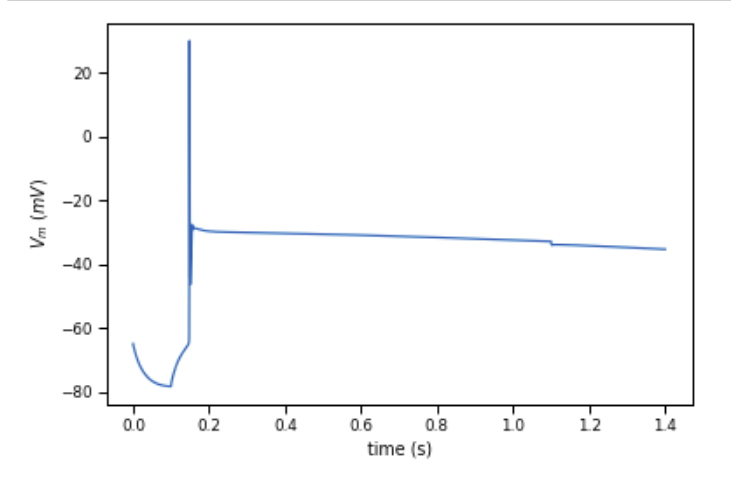
\includegraphics[scale=0.5]{figures/correct_active_l5pc.png}
    \caption{A current injection sufficient for causing a single spike is applied for a whole second from $100ms-1100ms$}
  \label{fig:sub1}
\end{subfigure}

\centering
\begin{subfigure}{.2}
  \centering
    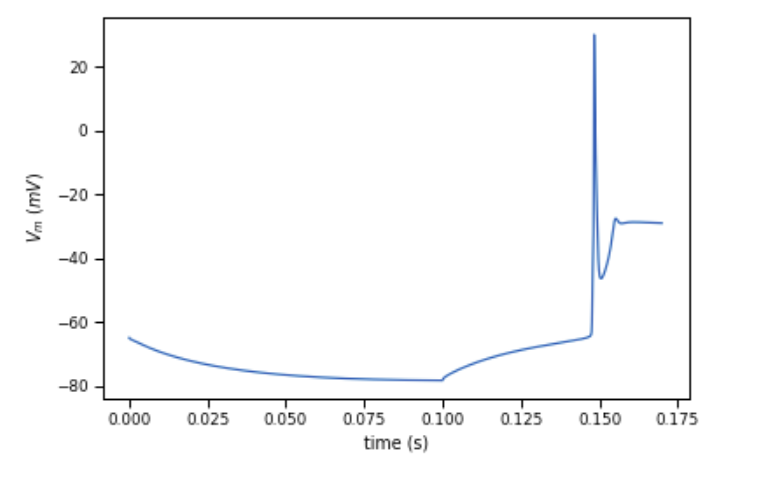
\includegraphics[scale=0.5]{figures/spike_shape.png}
    \caption{The spike shape is very brief in duration, and so it is worth zooming in for a closer look}
  \label{fig:sub1}
\end{subfigure}


\begin{subfigure}{.2}
  \centering
    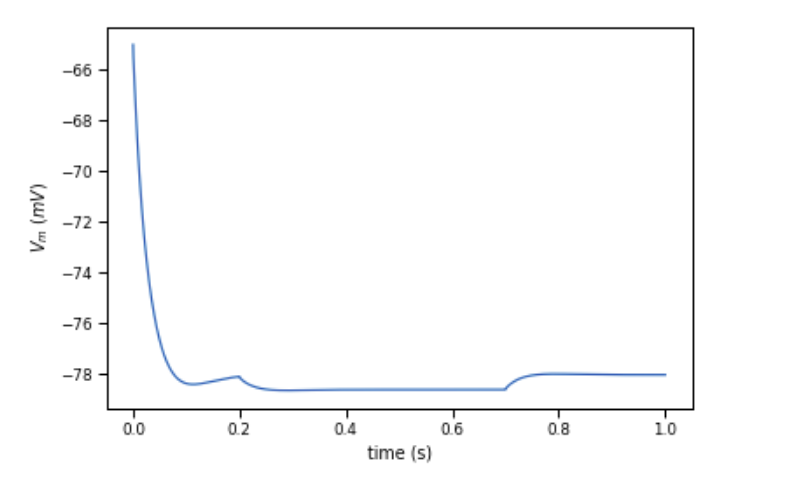
\includegraphics[scale=0.5]{figures/correct_passive_l5pc.png}
    \caption{A current injection value of -$10pA$ is applied to the cell for the duration of $200ms-700ms$}
  \label{fig:sub2}
\end{subfigure}
\label{fig:test}
\end{center}
\end{figure}


A test suite was constructed using NeuroElectro for the layer 4/5 Prefrontal Cortex pyramidal cell, and we were able to evaluate this layer 5 PC cells against the criteria of the neuroelectro test suite. 


\begin{table}[ht]
\centering
\resizebox{\textwidth}{!}{
\begin{tabular}{lllll}
\toprule
{} & observations &   predictions & Z-Scores & SEM \\
\midrule
RheobaseTest                   &    213.85 pA &      225.0 pA &  0.06542 & 128.868981 \\
InputResistanceTest            &  120.67 Mohm &  50.7 megaohm &  -0.9013 & 27.928023 \\
TimeConstantTest               &     15.73 ms &      16.76 ms &   0.1409 & 2.562106 \\
CapacitanceTest                &    150.58 pF &     330.66 pF &    1.289 & 1.488977 \\
RestingPotentialTest           &    -68.25 mV &     -78.04 mV &   -1.499 & 44.038610 \\
InjectedCurrentAPWidthTest     &      1.21 ms &       0.15 ms &   -1.979 & 0.174910\\
InjectedCurrentAPAmplitudeTest &     80.44 mV &      89.58 mV &   0.7174 & 1.488977\\
InjectedCurrentAPThresholdTest &    -42.74 mV &     -59.57 mV &   -2.094 & 1.922930\\
\bottomrule
\end{tabular}}
\end{table}
The corresponding statistics were
$(\chi^{2},p_{value})=(13.5609360364, 0.093951963105254)$

It is worth noting that the layer 5 neocortical pyramidal neuron was very slow to dispatch relative to the reduced models developed in this thesis work. Where as a typical reduced model described here evaluated in the order of $2.5 ms$, this model on average took $5.74$s, for a single run and $34.8$s to solve for the models Rheobase, current. To be fair, the model was run without activating NEURONs variable time step cvode. However, even with variable time step applied to the differential equation solver the magnitude of the disparity is still still several $seconds:$ several $ ms$. Neuroelectro lumps together, prefrontal cortex, somatosensory cortex and V1 PC cells together into a generic frontal cortex pyramidal cell model.

%The l5pc model was pre-optimized to fit to spike times and F/I mainly, and so it should not necessarily be expected to fit other electrical characteristics of the cell. Only the rheobase test, and the time constant test seemed to fall within the range of biological plausibility. None the less, this model remains a useful benchmark for reduced neuronal models.



%It was desirable to include this extended range of Izhikevich model behavior

%However, as noted in the introductory material, it i 


%Previously I mentioned neuronal modelling competitions I have optimize every model against the same data sets in order to assess overall which model is better able to fit to diverse data sets.



